\documentclass{article}

% if you need to pass options to natbib, use, e.g.:
% \PassOptionsToPackage{numbers, compress}{natbib}
% before loading nips_2016
%
% to avoid loading the natbib package, add option nonatbib:
% \usepackage[nonatbib]{nips_2016}

\usepackage{nips_2016}

% to compile a camera-ready version, add the [final] option, e.g.:
%\usepackage[final]{nips_2016}

\usepackage[utf8]{inputenc} % allow utf-8 input
\usepackage[T1]{fontenc}    % use 8-bit T1 fonts
\usepackage{hyperref}       % hyperlinks
\usepackage{url}            % simple URL typesetting
\usepackage{booktabs}       % professional-quality tables
\usepackage{amsmath,amsfonts,amsthm} % Math packages
\usepackage{nicefrac}       % compact symbols for 1/2, etc.
\usepackage{microtype}      % microtypography
\usepackage{graphicx}

\title{Social Networks Analysis using Compressive Sensing}

% The \author macro works with any number of authors. There are two
% commands used to separate the names and addresses of multiple
% authors: \And and \AND.
%
% Using \And between authors leaves it to LaTeX to determine where to
% break the lines. Using \AND forces a line break at that point. So,
% if LaTeX puts 3 of 4 authors names on the first line, and the last
% on the second line, try using \AND instead of \And before the third
% author name.

\author{
  Sahil Deshpande\thanks{Prof. Peter Chin
    Compressive Sensing and Sparse Recovery} \\
  Department of Computer Science\\
  Boston University\\
  Boston, MA 02115 \\
  \texttt{sahilsd@bu.edu} \\
  % examples of more authors
  \And
  Mikhail Andreev \\
  Boston University \\
  Boston, MA 02115 \\
  \texttt{mikh@bu.edu} \\
  \AND
  Chen Chen \\
  Boston University \\
  Boston, MA 02115 \\
  \texttt{takchen@bu.edu} \\
  \And
  Stephanie Chiao \\
  Boston University \\
  Boston, MA 02115 \\
  \texttt{schiao@bu.edu} \\
}

\begin{document}
% \nipsfinalcopy is no longer used

\maketitle

\begin{abstract}
Social Networks are well-known for their massive scale. Analyzing the social networks to extract meaningful information
is one of the most significant aspects of managing such massive user data. Larger the data, more valuable is the
extracted information. But such scale of data is not always an advantage. When social networks have billions of nodes
and relationships, the traditional graph algorithms that run in polynomial time pose a significant disadvantage for
analyzing the social networks. Therefore, in this paper, we will try to find ways to apply compressive sensing to social
networks. The idea is to find some set of sparse characteristics in a social network that allows us to group the users
together and makes it easier to analyze the entire social networks in groups.

\textbf{Index - } compressive sensing, social networks, inter-community detection.
\end{abstract}

\section{Introduction}
Graphs have always been an efficient way of representing large amount of data. The nodes stand for individual entities
and the edges represent some non-trivial relation between them. This idea has been extended to represent billions of
users and their mutual relationships in the real-world systems such as social networks [7]. A typical representation of
social networks using graphs, or social graphs, is to represent the users as nodes and their relationships such as being
friends, accessing similar content is represented by edges. The edges can further have some weights associated with them
to denote the degree of associativity between the users. Such structural representation can often blow up in size. It
becomes very difficult to look at all the nodes and edges to quickly retrieve any meaningful information. Something as
simple as finding top $k$-nodes can take order of few minutes using polynomial time algorithms. 

To avoid this problem, it's sometimes easier to group the nodes together and analyze the clusters of multiple nodes
together. This shrinks down the problem of analyzing billions of nodes to analyzing a few hundred or thousand nodes
depending on the degree of such clustering. Such groups, or $communities$ of users correspond to the real-world social
groups [2]. This makes such groups even more significant because of the important characteristics it stands for. These
communities are the more intensely connected groups with relatively small number of edges between them. In this paper,
we try to analyze applications of compressive sensing to identifying these small number of important edges that connect
multiple communities. Naturally, by treating the graph as a signal, the problem gets converted into that of retrieving
some $k$-sparse vector corresponding to $k$ such edges [1]. 

The rest of the paper discusses brief background and current scenario of applications of compressive sensing to social
networks in section 2. Then we take a closer look at one such algorithm called LSR-weighted in section 3. Then section 4
discusses various real-world applications to utilize such community detection. Section 5 describes the results of
running LSR-weighted and shows how these communities look by 3D visualization. Then we conclude by looking at important
characteristics and limitations of these algorithms and mention few possible enhancements. 
\section{Related Work}
Within past decade, online social networks have emerged and have given a new dimension to complex graph networks. For
example, according to Nielsen [2], worldwide users spend over 110 billion minutes on social media sites per month, which
accounts for 22\% of all the time spent online, surpassing even the time spent on email. In the analysis of social networks, the existence of missing data is almost inevitable because the aforementioned constraints may prevent access to entire data of the networks. Mostly, direct measurement of each individual node can be difficult, costly, and sometimes impossible due to massive scale, distributed management, and access limitation of real social networks.

The developments in compressive sensing started with the seminal works in [1]. The authors noted that the
combination of l1-minimization and random matrices can lead to efficient recovery of sparse vectors and also has
strong potential to be used in many applications. For the last couple of years, CS has been considered in signal
processing, but its role in network applications is still in its early stages due to some challenging issues [3]. In
networks, measurements are restricted by network topological constraints which is again absent in existing CS research.
In other words, for every measurement, only links that induce a path or connected sub-graph can be aggregated together
in the same measurement [5]. As a result, compressive sensing for network applications is quite different from other CS problems, although it is interesting in its own right because we can represent many real-world systems by their graphs/networks.

The first paper we found that applied compressive sensing to large graph networks was [3] which used compressive sensing
to computer networks to identify congested links that are vulnerable to packet drops. This research falls under the
category of $network\ tomography$ and states many theoretical constraints on using traditional compressive sensing
techniques on graph networks. The algorithm proposed is quite efficient and serves the purpose of monitoring computer
networks. But the main disadvantage it has is the biased output due to a technique called random walks. While randomly
traversing the graph, the algorithm is biased towards nodes of high degree. So it fails to capture the weighted
unbiasedness in a network.

This lack of weighted constraint is solved solved by considering weights while traversing the graph in [6]. This
algorithm is also equally efficient and talks about important null-space property of measurement matrix which guarantees
correctness on the algorithm. But this algorithm doesn't talk about the applications of Compressive Sensing in Social
Networks. This topic is discussed in detail, probably for the first time, in [4]. This work describes how we can
overcome the theoretical challenges discussed in [6] while enabling weighted unbiased output for detecting
inter-community structures. The paper also briefly describes a relatively new $l1$-minimization technique called Lasso
[9]. This algorithm is very similar to LSR algorithm which is described below.  
\section{LSR Algorithm}
LSR stands for low-cost sparse recovery framework. It takes advantage of the sparsity property in social networks, which in most cases, are graphs represented by nodes and edges. Sparsity is a natural assumption in some social network analysis such as the detection of inter-community links in social networks and identification of top-k central nodes in networks. Because the number of such nodes and links are much smaller than the set of all nodes and links in networks.

There are two constraint worth mentioning in this field
\begin{itemize}
\item Measurement matrix is in a more restrictive class taking only non-negative integer entries, while random Gaussian measurement matrices are usually used in CS literature.
\item Network topological constrains which is not considered in existing CS researches.
\end{itemize}
And there are a few recent works that do consider the network topological constraints in order to construct a feasible measurement matrix. But the problem is they don’t take into account the strength of links, which is definitely not realistic. The previous works include the state-of-the-art CS-based algorithms ,RW, and UCS-WN.
LSR-weighted algorithms improve the functionality in the following two major aspects
\begin{itemize}
\item A feasible measurement matrix with less number of measurements and relative low-error
\item Maximum coverage of network
\end{itemize}


\subsection{General Model}
The general model is:
$$y_{m\times} = A_{m \times |E|}x_{|E|\times1}$$
input for the algorithm is the graph ,and the output is the A measurement matrix. Here is an A matrix from a random graph that can give you better intuition about what it is:

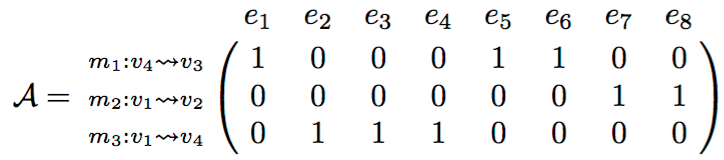
\includegraphics{A_matrix.png}

so in this example, we have 3 rows, which means 3 measurements, and each measurement is an iteration of the algorithm, and at the same time, it is also the traversal of a certain part of the graph. The number of columns denotes the number of edges in the graph.


Besides, we represented the graph using upper adjacency matrix, and all the functions and operations we wrote are all based on the property of upper adjacency matrix.


The edge index of the graph is simply defined in this way: it starts from the
(1,2) to (1,3) to (1,4) to (end of row), then start from the (2,3) to (2,4) to (end of row),etc. This is basically like a snake.








\section{Applications}
With this algorithm, it's easy to identify the inter-community edges that define some clustered graph structure. Till
now, we've seen that a graph can represent multiple types of relations. By interpreting the edges in various ways, we
can use this same algorithm to group the users by different heuristics and extract different types of information. We
discuss a few possible application here.
\subsection{Friend Recommendations}
The relationship between two users can be that of friendship. This relation itself can be described using two different
entities of weighted and unweighted edges. If we define friendship relation exists if two users are online friends, it's
unweighted relation. If we describe the degree to which they've mutual online friends, then it becomes a weighted graph
with weight of the edge describing the degree of connectivity. By running LSR-weighted on such graph, we can easily
group the users together. Such communities can then be used to suggest friends within the same community or across
different communities. 

\subsection{Advertising Content}
By representing the edges as the degree to which users access similar content, we can group the users together based on
accessed content correlation. If this content is specifically the advertisements that users found relevant, then we get
an interesting clustering of users based on similarity of advertisements. It can help targeted advertising [10] where
users from the same community can get similar advertisements to optimize the user experience and in turn increase
revenue.

\subsection{Detecting Filter Bubbles}
Social networks have been under close scrutiny for filtering the content according to what the user wants rather than
exposing variety of content. By using this data of accessed articles, videos, photos, etc., we can identify groups of
people who are restricted to a small subset of the shared data. Using these clusters, we can further suggest data
consisting of different view points than what the community is restricted to.

\subsection{Detecting False Information}
Suppose we identify the groups of users interested in similar type of content. If we rely on users to notify this false
information, there is a good chance that users that disagree with valid information might report it as false information
just to discourage that source. Instead, we can aggregate this user input across different communities and effectively
identify the real false information sources. 

There could be plenty more applications where analyzing a cluster of users can be more effective and efficient rather
than looking at individual user. These are small subset of such applications that could be extended further as more
sophisticated approach to solve the corresponding problems.  
\section{Results}
Using the algorithm presented above, we evaluated it on several datasets. Our data included both previously compiled data as well as real-world examples compiled specifically for this project. Here we will explain the structure and source of our datasets, then we will show the results and present our analysis of those tests.

\subsection{Dataset}
There are three primary datasets we tested the algorithm on. All of these datasets are real-world weighted social networks with different sets of links. The first dataset is the network of personal relationships via the Freeman EIES System which has been examined in previous papers. Our other two datasets come from a popular social media and forum discussion website known as Reddit. 

\subsubsection{Reddit Datasets}
The Reddit platform consists of a series of forum pages on which users can post submissions and comment on other people's submissions. This allows users to demonstrate their interest in a variety of topics, as each forum page is dedicated to a specific topic. A users posting and comment history is publically available. Taking advantage of this, we crawled the Reddit's pages, and acquired a list of users who have made comments on those pages. From there, we linked back to the user, and acquired a list of the pages that the users posted on. If a user had a large number of posts on a specific forum's page, this was a clear sign of interest in that topic. Using this scheme, we constructed a relative interest chart for each user. We then correlated the users based on shared interests to create a weighted graph. Each node represented a user, and each edge was the amount of shared interest two users had. 

Using this as the base data-set, we constructed two types of graphs to view the relationship between users. The first type of graph consisted of random users chosen from the datasets with a set number of links between them. Since the users present here was random there was no intrinsic structure to this type of graph. The second type of graph involved taking users who predominantly posted to one of the pages. After acquiring several such groups of users, we examined the the links they had in-between the different groups. Since the user's primary interests were not related, the links between users in two different groups were much weaker than those within a single group. From here we ran the algorithm to see if we could decrease the graph complexity while still retaining the inter-graph connections.

\subsection{Visualization}
In order to better understand the sparse structure of the graphs, we created a visualization engine that would plot the different networks overlayed with the sparse structure. In an effort to acquire groupings for the non-grouped data, we ran the datasets through a K-Means grouping algorithm and used those groups in the display.

\subsection{Graphs}

\subsection{Results}

\subsection{Analysis}

\section{Conclusion}
In this paper, we've looked at compressive sensing as an effective way of handling massive scale data in social
networks. We discussed the major theoretical limitations faced by compressive sensing in social networks analysis. Along
with LSR-weighted algorithm, we also looked at various approaches studied so far. The implementation of LSR-weighted
also produces some encouraging results seen in the results section after running the algorithm on real-world dataset
from reddit [?]. The main limitation we've found here is the
coherence in social network. When we've a sparse network, the measurement matrix can be empty where we fail to output
any sparse edges. But overall, it works well and there are some interesting applications as well to utilize this
information of clustered users. 

\section{Acknowledgements and Credits}
We would like to thank Prof. Peter Chin for helping us understand the problem statement and giving a few basic ideas to
begin investigation. The techniques taught during CS591C2 course were also helpful during this project. 

For most of the project, we worked together as a group. A rough distribution of work can be seen as follows, \\
Sahil - initial research involving going through a few papers, help with coding, applications of LSR-weighted \\
Mikhail - Acquiring real-world data, visualization, and testing\\
Chen - Implemented the first and second version of LSR algorithm \\
Stephenie - Joined the group after most of the ground work was done. Assisted in data compilation and results analysis.

\section*{References}
\small

[1] D. Donoho, “Compressed sensing,” IEEE Trans. Inf. Theory, vol. 52,
no. 4, pp. 1289–1306, Apr. 2006.

[2] Nielsen statistics and measurements, june 2010. [Online].
mobile/social-
Available: http://blog.nielsen.com/nielsenwire/online
media-accounts-for-22-percent-of-time-online.

[3] J. Haupt, W. Bajwa, M. Rabbat, and R. Nowak, “Compressed sensing
for networked data,” IEEE Signal Processing Magazine, vol. 52, no. 2,
    pp. 92–101, Mar. 2008.

[4] H. Mahyar, H. R. Rabiee, Z. S. Hashemifar, and P. Siyari, “UCS-WN: An
Unbiased Compressive Sensing Framework for Weighted Networks,” in
Conference on Information Sciences and Systems, CISS 2013, Baltimore,
USA, Mar. 2013.

[5] M. Wang, W. Xu, E. Mallada, and A. Tang, “Sparse recovery with graph
constraints: Fundamental limits and measurement construction,” in IEEE
INFOCOM, Mar. 2012, pp. 1871–1879.

[6] W. Xu, E. Mallada, and A. Tang, “Compressive sensing over graphs,”
in IEEE INFOCOM, Apr. 2011, pp. 2087–2095.

[7] Reddit - www.reddit.com

[8] H. Mahyar, H. R. Rabiee, A. Movaghar, E. Ghalebi,
and A. Nazemian, “CS-ComDet: A Compressive Sens-
ing Approach for Inter-Community Detection

[9] R. Tibshirani, “Regression shrinkage and selection via
the lasso,” Journal of the Royal Statistical Society B,
vol. 58, pp. 267–288, 1994.

[10] https://en.wikipedia.org/wiki/Targeted\_advertising


\end{document}
